\documentclass[12pt, letterpaper]{book}

\usepackage{imakeidx}

\usepackage[obeyspaces]{url}

\usepackage[english]{babel}

\usepackage[backend=biber]{biblatex}
\usepackage{csquotes}
\addbibresource{references.bib}

\usepackage{graphicx}

\usepackage{hyperref}
\hypersetup{
    colorlinks=true,
    linkcolor=blue,
    filecolor=magenta,      
    urlcolor=cyan,
    pdftitle={Overleaf Example},
    pdfpagemode=FullScreen,
    }

\usepackage{amsthm}
\newtheorem*{remark}{Remark}

\title{Tomb Editor Manual}
\author{rickyturaz}

\makeindex
\begin{document}

\maketitle
\tableofcontents

\part{Introduction}
\chapter{History of Tomb Raider Level Editors}
\section{Back to 2000: \emph{Tomb Raider Level Editor} \index{Tomb Raider Level Editor}\index{TRLE}}
Tomb Raider marked a sensational new approach to 3rd person gaming. Fans not only fell in love with Lara and her moves, but with the imaginative and intriguing worlds of her adventures. It all started with Lara's visit to some Egyptian ruins back in 1996, and now with the release of the Tomb Raider Level Editor has come full circle, offering a different sort of adventure in another Egyptian setting. \emph{Tomb Raider Chronicles} marks the end of the line of Tomb Raider games made with these development tools; but rather than viewing this as an end, the release of the editor makes it seem more like a beginning...
\par The \textbf{Tomb Raider Level Editor (TRLE)} includes a tutorial that will walk you through the basics needed to create your own stand alone Tomb Raider levels (but please read the legal disclaimer about commercial use of this product). Even though you will not be able to edit objects or animations (that means Lara’s outfits), you have a wonderful variety of object sets from which to choose. You can sculpt and design on many different ‘levels’ – trigger events, create awe-inspiring spaces, simple to complex…and as you experiment you will learn more about what can be done, and quite possibly discover new methods of applying the knowledge you have acquired.
\par We sincerely hope you will enjoy inventing, designing, and building with and for Lara as much as we have over the past 4 years. We thank all those who have held the enthusiasm for the Tomb Raider series, thereby contributing to its success. We wish you happy adventuring with Lara and the tools used to create her worlds.
\cite{trle_manual}
\section{Paolone's \emph{Next Generation Level Editor} \index{NGLE} \index{Next Generation Level Editor}}
The \textbf{Next Generation Level Editor}, often abbreviated \textbf{NGLE}, is a modified version of the Tomb Raider Level Editor, created by Paolone, and released in January 2007. \cite{wikiraider_NGLE}
\par Tomb Raider Next Generation \index{Tomb Raider Next Generation} (TRNG) \index{TRNG} tools, improve the TRLE tools used to build custom levels with the engine, supplied by Eidos, of Tomb Raider - The Last Revelation.
\par Many objects have beed added, some imported by other TR adventures, like boat or frog-man, other builded ex-novo like Detector or Elevator.
\par There is a new scripter program named NG\_Center. This program other to build your script.dat supplies other little tools. \cite{paolone_trng}
\section{MontyTRC89's \emph{Tomb Editor}}
\textbf{Tomb Editor (TE)} is a level editor designed for the full range of classic Tomb Raider game series (1-5), as well as for contemporary engine reimplementation projects and game engines designed for community modding and level building. \cite{TE_github}

\chapter{Basic concepts to know about Tomb Raider}
% Inserire qui i concetti fondamentali relativi a Tomb Raider, da sapere. Ad esempio, se parlo di TR4 devi sapere di cosa si parla. Scherzaci un po' su: se sei qui a leggere questo manuale, un po' Lara ti deve piacere, no?! :)
\part{Getting started}
\chapter{Installing Tomb Editor}
First of all, you need to download and install the Tomb Editor pack on your computer. wIt is available eg. \href{https://tombengine.com/}{here}.
\par The default route of Tomb Editor installed is \path{C:\Tomb Editor}. The contents of this main folder are:
\begin{itemize}
    \item Tomb Editor program.
    \item Side programs dedicated to Tomb Editor: SoundTool, TombIDE, WadTool.
    \item Most of the files which are necessary to start a basic project and level for Tomb Engine. (But texture files for room faces must be find somewhere else. But this is still not necessary now, when you start reading this tutorial.)
    \item Other important files for Tomb Editor pack.
\end{itemize}
So when you have the Tomb Editor pack installed on your computer, then you are just ready to start building levels for Tomb Engine. \cite{akyv_tutorial}

\chapter{Starting a new project}
After the installation of Tomb Editor pack, you are ready to make your very first Tomb Engine project. (Level map file extensions are well-known as “PRJ” files, but do not misunderstand: what we call “project” now is not a level, but a whole level set - i.e. your current Tomb Engine game itself, which will be released when you fully made it.)
\par But where do you need to place your projects? Well, NOT in Tomb Editor main folder - that is a place you usually never modify while editing. I suggest placing all of your projects nicely collected in a so-called general project folder. This could be called eg. \path{"My_Tomb_Raider_projects"}, created manually. (I created it in Documents folder.)
\par Each project you make will be placed in its own main folder. Does it mean now you should also create manually a project main folder in the general folder? No, there is a TombIDE wizard which will do the whole project-creating procedure for you.
\par Projects are handled in \textbf{TombIDE (Tomb Integrated Development Environment or TIDE)} program, that is why the whole project-creating procedure is also being done there.
So start \path{TombIDE.exe}, and the panel of TIDE Start page opens up.
Click on “Create a new project” button now.
The first page of a new panel opens up (General Information, \ref{fig:tide1}):
\begin{figure}
    \centering
     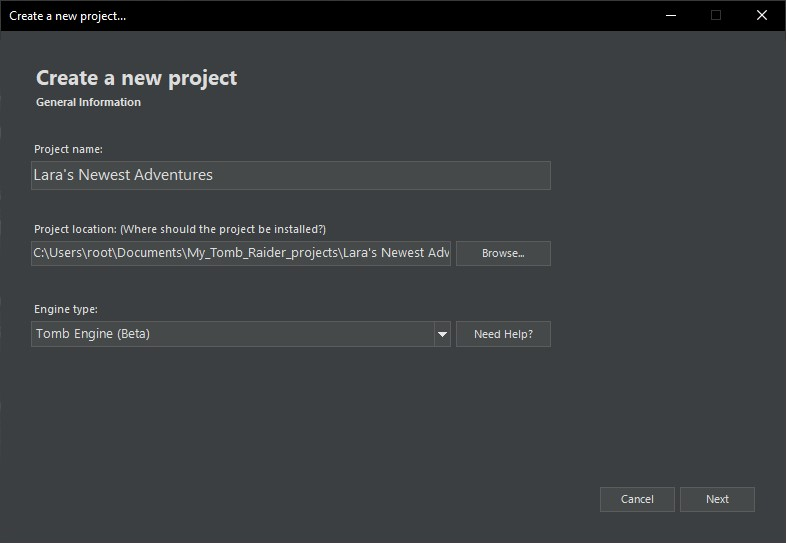
\includegraphics[width=0.75\textwidth]{screenshots/1.jpg}
     \caption{General Information}
     \label{fig:tide1}
\end{figure}

\begin{itemize}
    \item Let's suppose the project you start now has the name of “Lara's Newest Adventures”. So type it now here.
    \item Click on “Browse” button, find and select the general project folder.
    \item After that, the little window in the middle of this first page shows that a subfolder in the general project folder will be created as the main folder of this project, having the project name.
    \item The engine type you choose now is naturally Tomb Engine.
\end{itemize}


\par Now click on “Next” button to continue the procedure on the next page of the panel (Extra Options, \ref{fig:tide2}).

\begin{figure}
    \centering
     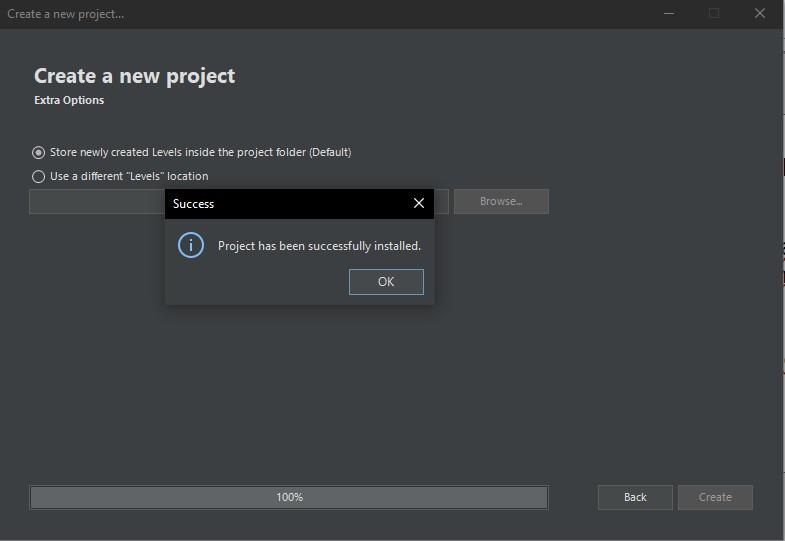
\includegraphics[width=0.75\textwidth]{screenshots/2.jpg}
     \caption{Extra Options}
     \label{fig:tide2}
\end{figure}

\par I suggest changing nothing here. Which means level map files will be handled in a folder called "Levels", which is a subfolder in the main folder of the project. (I mean, this is the default place for level map files, and you, the beginner probably should keep it like this.)
\par Now click on "Create" button here, then look at the increasing bar at the bottom of the panel.
When the bar is at 100 \%, then you get a message that the project has been successfully created (\ref{fig:tide3}).

\begin{figure}
    \centering
     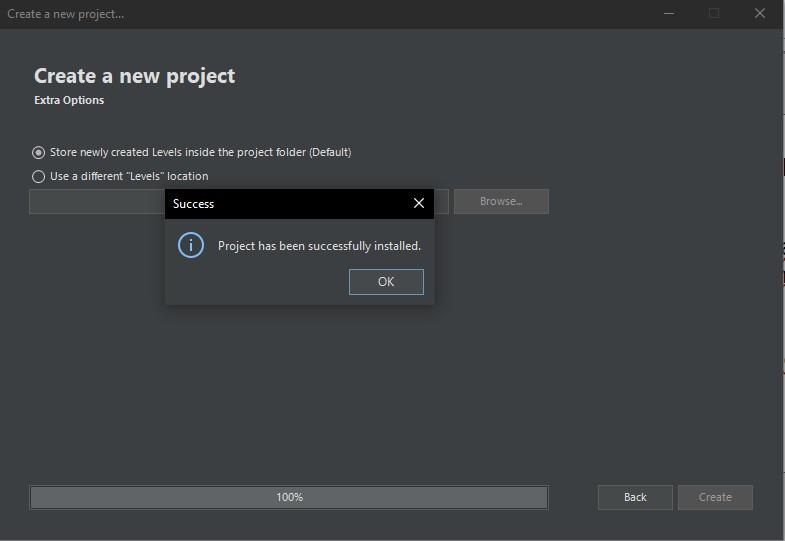
\includegraphics[width=0.75\textwidth]{screenshots/3.jpg}
     \caption{Project has been successfully installed}
     \label{fig:tide3}
\end{figure}

\par And this project main folder has been also created on the selected route, with the basic contents a TEN project should have. (Including Levels folder - still being empty - in that default position., \ref{fig:tide4})

\begin{figure}
    \centering
     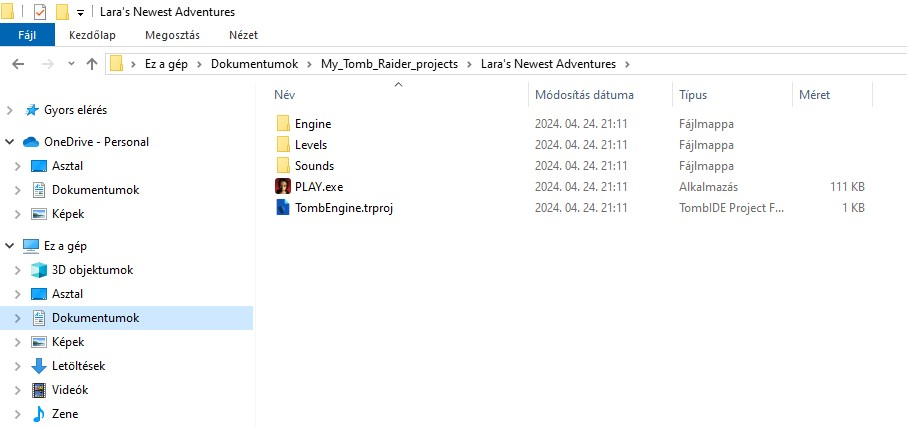
\includegraphics[width=0.75\textwidth]{screenshots/4.jpg}
     \caption{Project directories have been created (Since TEN 1.7., the project main folder has an Assets subfolder as well.)}
     \label{fig:tide4}
\end{figure}

Double-click on that row (or click on "Open selected button" below), so the project opens in TIDE, you will be able to work on it. Each project opened in TIDE has more pages, now you can see its Level Manager page. (See the panel header which names the current project.)
\par Now click on the red arrow in the upper left corner of the page, to go back to TIDE Start page, closing this project now in TIDE. (Since TEN 1.7., you can see the blue TIDE icon in that corner, instead of the red arrow. If you click on that icon, then a menu opens. One of the menu options is an arrow, with "Back to Start Window..." name. Click on it to go back to TIDE Start page.) \cite{akyv_tutorial}
\part{Principles of game development}
\chapter{Beta testing}
\section{In General}

Beta testing is perhaps the most important phase of any video game's development. Whether you've spent a month or a few years on your adventure, if you don't have it beta tested properly, all that work could be ruined by one simple little gameplay killer. If you understand the importance of beta testing, then read this tutorial carefully and take it to heart. \emph{If you don't understand the importance of beta testing, then read this tutorial carefully and take it to heart.} I cannot stress enough how important the beta testing phase is.
\par When should beta testing begin? The short answer is after alpha testing is finished. When is alpha testing finished? That's easy! That's when you think your game is ready for release. Your game is the best you can get it and you're sure there is no more you can do and you feel happy about releasing it. Now it's time for beta testing. This seems to be a difficult concept for new Level Builders (and a few seasoned Level Builders) to get their heads around. Trust me, your game does not go for beta testing until you are convinced it's finished. If it's not finished, you're still in the alpha testing stages and if you employ your beta testers now they will be wasting their time and your game will not be beta tested properly.
\par When a game moves from alpha testing to beta testing, the only changes you should make would be to fix bugs, gameplay errors and textural errors. You should never build new areas or new gameplay or new puzzles during or after beta testing. Again I stress, do not begin beta testing until your game is FINISHED. Beta testing is purely to iron out problems in finished games. If you ignore this advice the chances are you will release a buggy game. Beta testers take their job seriously and if games are released with bugs it reflects on them and the job they did. If those bugs are down to the Level Builder changing things during or after beta testing and the game is released with bugs you will never get beta testers to help you again. Beta testers will invest days and even weeks of their personal time to help you with your game. Respect that and don't let them down.

\section{Alpha Testing}
Don't cut corners and skip this step. Yes, I know, you're excited about your game and you want to show it off and that's marvellous and wonderful and admirable and quite understandable, but your beta testers are not there to do your job for you. If you upload an appallingly buggy game that hasn't been properly alpha tested, don't be surprised if your beta testers don't do a good job and don't volunteer later when you actually need beta testers. Alpha testing is your job, not your beta testers, and it's extremely important. I consider my alpha testing to be complete when I have a package I think is ready for release. In other words, I can find nothing to change or fix and in my heart I know my game is the best I can make it and I feel it's ready for release. Now I begin beta testing.
\par During alpha testing, it is easy to move Lara around and forget to put her back, place temporary triggers to open a door and then forget to remove them and a few other little things, so after I've packaged up my game for beta testing guess what? Yes, I then test the beta package from start to finish using only the files I will be uploading for my beta testers. This is my final Alpha test. If this goes well and all the level jumps work properly and I successfully hit a finish trigger, only then is the game uploaded and the download link sent out to the beta testers.

\cite{NGLE_manual_hu}

\printindex
\printbibliography
\end{document}